\cleardoublepage%
\chapter{\label{chap:res}Results and Discussion}%

%This is where you present your findings. As much as possible, structure your results along the lines of your research questions. Start with the simplest results first and proceed to more complex ones. Tables and Figures should be clear enough that they need little explanation: do not simply re-write the numbers as text to fill space. Rather, highlight trends, outliers, or gaps. 

\section{\label{sec:res_networking}Networking}%should this be in firmware?

As described in Section \ref{sec:methods_net_des} and Section \ref{sec:methods_net_dev}, and in line with research question 1, a networking structure has been designed and developed for use with the Smart Motors-based hardware.

\subsection{\label{sec:res_logic}Concept, Structure and Logic}

As outlined in Section \ref{sec:methods_net_des} and Section \ref{sec:methods_net_dev}, the networking was designed and developed in two parts, the Networking Library and using the interfaces of the base networking as a base, the more specific SSP Add-on Library. \\

The Networking library is designed to be a general purpose library that builds on ESP-NOW and adds some basic structure and functionality. This base networking introduces address book logic that bypasses ESP-NOW's 20 peer limit, allowing transmission to a theoretically unlimited number of peers at the expense of efficiency. It also introduces the basic message structure, including different message types (cmd, inf, ack) and different subtypes (cmd: ping, echo, boop; inf: msg, data; ack: pong, echo, boop). The library also includes logic to send data larger than $241\ bytes$, the maximum payload allowed using the message structure defined in Section \ref{sec:rev_net}, increasing it to a theoretical limit of $60'928\ bytes$. However, in reality the message limit is lower, with the maximum amount successfully transmitted at about 30 kB due to the memory limitations of the MicroPython firmware running on the ESP32C3. Also, sending large messages in chunks runs the risk of some chunks being lost during transmission (see Section \ref{sec:res_rssi}), especially over long distances, resulting in the entire message being dropped. While there is a provision in the code to remedy this by storing all parts of a long message in a buffer, and if the receiving device is missing one or more parts of a multi-part message after some time, it sends a message requesting the missing parts, this has been disabled for memory optimisation. 
The network design also includes various interfaces for customisation and the addition of additional custom commands, message types and handling logic, including custom IRQ messages. \\

Building on top of these interfaces of the base Networking Library, the SSP Networking Library introduces many additional smart module specific commands, handlers and message types, which allow the effective control and configuration of smart modules using the appropriate commands. The specific structure of the code of the two libraries and all their commands are shown in Figure \ref{fig:net_code_structure}.

% \begin{figure}[H]
%     \centering
%     \includegraphics[width=.5\linewidth]{overleaf/images/placeholder.png}
%     \vspace{\ftspace}
%     \caption{Networking overview}
%     \label{fig:Networking overview}
% \end{figure}

As such, the Networking Library meets all the requirements outlined in Section \ref{sec:methods_net_des}. In particular, it is compatible with the Smart Motors hardware and with any ESP32-based hardware that includes Wi-Fi and thus ESP-NOW capabilities, as well as with the MicroPython firmware used. The protocol uses a peer-to-peer communication approach, inherited from the basic ESP-NOW design on which it is based, and requires no central root or hub or even configuration to use, other than initialising the library. It also includes message validation features, using a common message structure that includes an identifier and checksum, and provisions for easy module discovery, using the ping command defined in the base Networking Library, and interaction, using the various further defined commands and message types defined in the SSP networking add-on, which further satisfies the latter two requirements. In terms of design principles, the networking is split into two parts, allowing the base networking, which contains simple logic and commands, to be used in a variety of custom ways, and further allowing interfaces for customisation. The code is furthermore following the style Guide for Python Code based Python Enhancement Proposal 8. \citep{rossum_python_2001}

\subsection{\label{sec:res_range}Range Test}

As outlined in Section \ref{sec:methods_test_range}, the original range test was conducted using the boop-o-meter program on a street in front of the CEEO offices. The maximum range at which some messages were still being received by each of the two modules was approximately 242 meters, as shown in Figure \ref{sec:res_range}.

\begin{figure}[H]
    \centering
    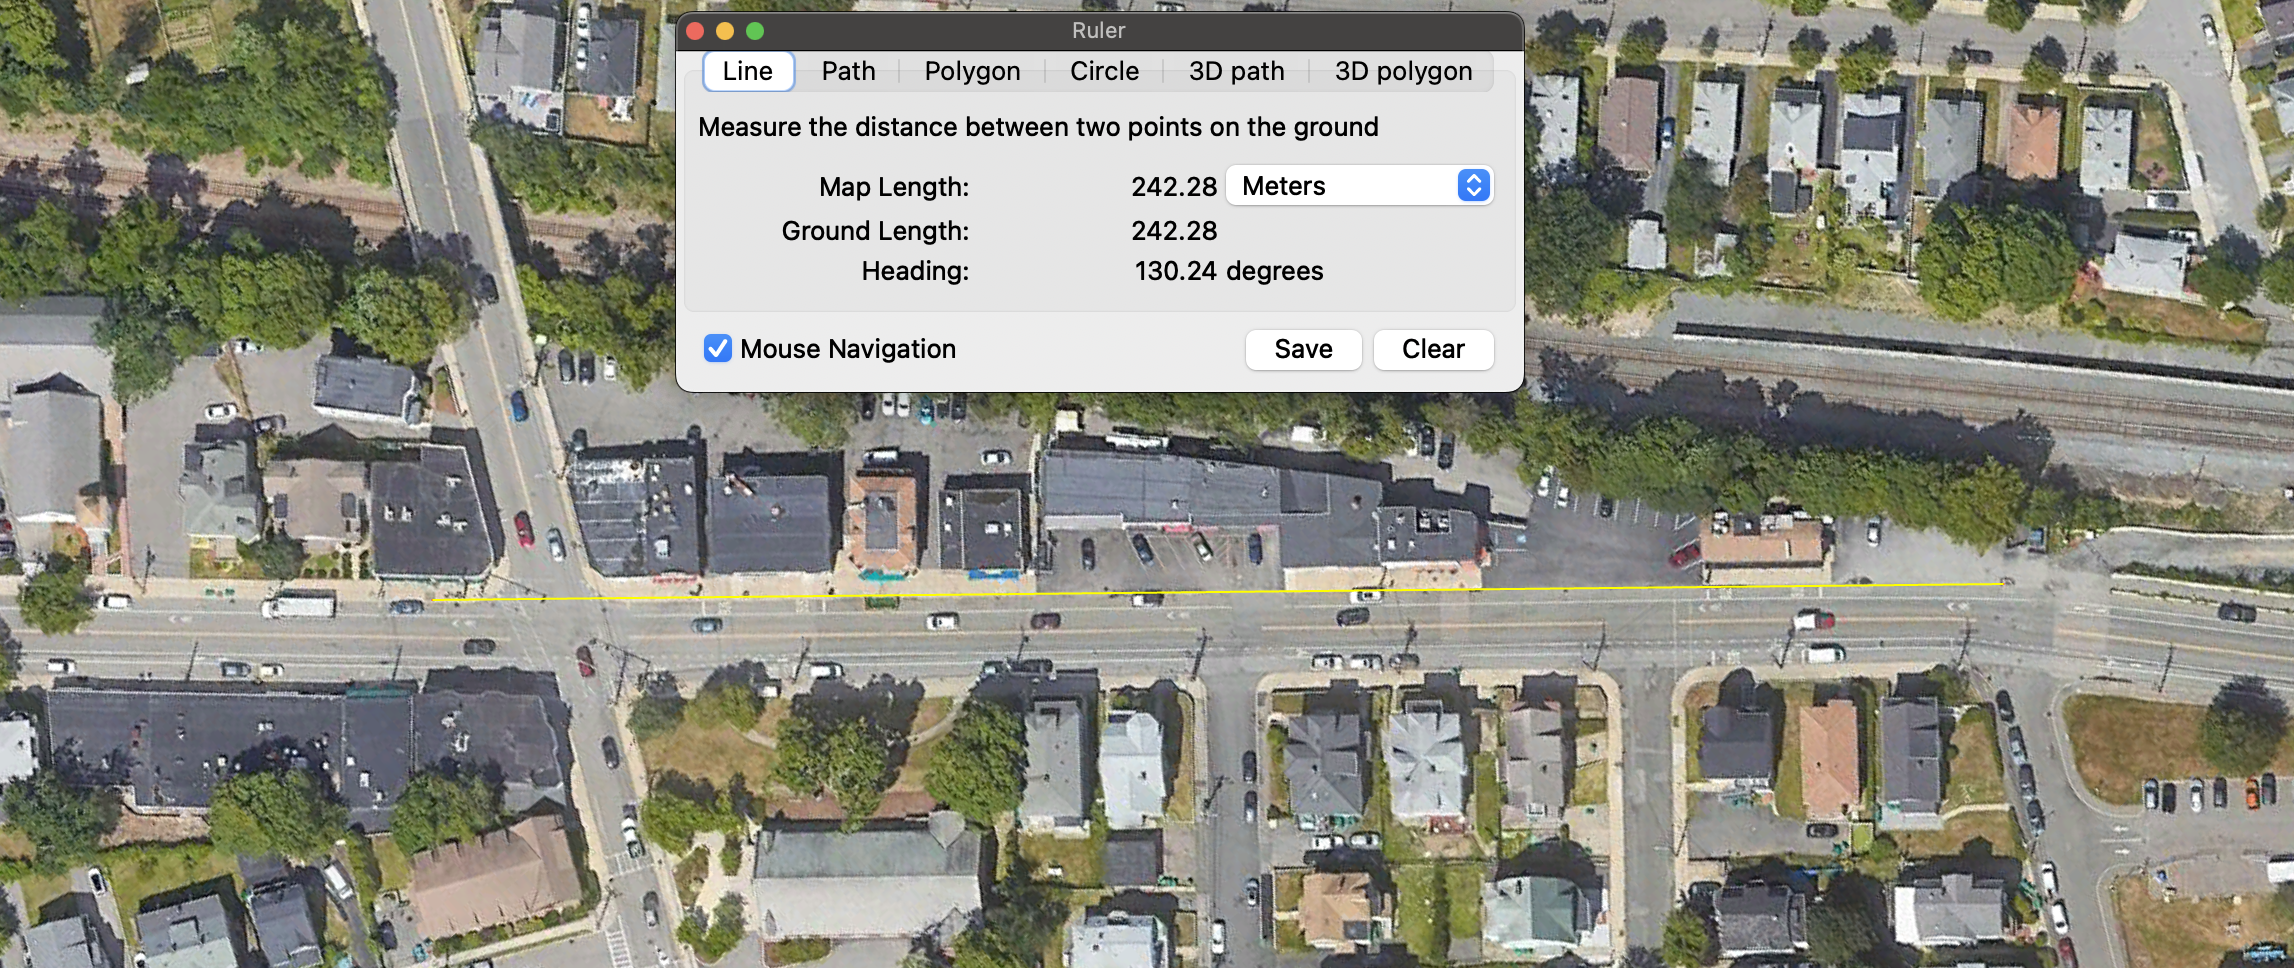
\includegraphics[width=\linewidth]{overleaf/images/range.png}
    \vspace{\ftspace}
    \caption{Approximate range test on Boston Avenue, MA}
    \label{fig:range}
\end{figure}


\subsection{\label{sec:res_rssi}Response Time, RSSI and Packet Loss Rate by Range}

The RSSI, ping response and packege loss for various ranges was measured three times using two ESP32C3s, one ESP32C3 and one ESP32C6 and again using two ESP32C6s.

\subsubsection{ESP32C3 to ESP32C3}

As expected, the RSSI values, an index for signal strength, drops for longer ranges, following a logarithmic curve, as shown in Figure \ref{sec:res_rssi}. The RSSI values for both devices are very similar and also follow a similar curve, with a slight divergence, which could be explained by differences in production quality of the antenna.

\begin{figure}[H]
    \centering
    \begin{subfigure}{0.45\textwidth}
        \includegraphics[width=\linewidth]{rstudio/analysis/plots/ESP32C3_rssi_box.png}
    \end{subfigure}
    \begin{subfigure}{0.45\textwidth}
        \includegraphics[width=\linewidth]{rstudio/analysis/plots/ESP32C3_avg_rssi.png}
    \end{subfigure}

    \begin{subfigure}{0.45\textwidth}
        \includegraphics[width=\linewidth]{rstudio/analysis/plots/ESP32C3_ping_box.png}
    \end{subfigure}
    \begin{subfigure}{0.45\textwidth}
        \includegraphics[width=\linewidth]{rstudio/analysis/plots/ESP32C3_avg_ping.png}
    \end{subfigure}
    \vspace{\ftspace}
    \caption{RSSI and Ping time depending on antenna angle}
    \label{fig:rssipingrange_esp32c3}
\end{figure}

In terms of ping time, the averages are not affected by range, which makes sense as the increase in travel time from 0 to 100 meters is only approximately $0.0000033356\ ms$ ($100\ m\ /\ 299'792'000'000\ m/ms$), which is insignificant compared to the time taken by the MCB to process it. Interestingly, the values tend to cluster at specific values with a distance of $10\ ms$, either $10\ ms$, $20\ ms$ or $30\ ms$, which might be caused by an underlying system clock rate of the MCB. There are various outliers in terms of ping time, more notably for the larger distances, though also for the measurements at 1 and 0.5 meters. The outliers of these two measurements were the first measurements of the tests, both likely taken after a restart of the used ESP32 MCBs. As such, the code had to add the peer it received the message from to its ESP-NOW buffer, which might explain some of the delay and the high ping response time for the first measurement. Subsequent measurements taken at the same distance, for example for the angle tests in Section \ref{sec:res_angle}, did not yield any such outliers, however most measurements after restart of the device, did. For other test sessions the code was usually tested in a first trial run, whose data was disregarded, which might be why this is only apparent for these two specific measurements.

As for packet loss, transmission remains lossless until 25 meters, at which point packets start to become lost. These values increase with distance, with about one third of packages lost at a distance of 100 meters, as shown in Table \ref{tab:rssipingrange_esp32c3}.

\begin{table}[H]
    \centering
    \begin{tabular}{|c|c|l|l|c|c|c|c|c|}
    \hline
        Range & Packet Loss & \multicolumn{2}{l|}{Measurement} & \multicolumn{5}{c|}{Values} \\\hline
        [meters] & [\%] & \multicolumn{2}{l|}{} & mean & std & min & max & median \\\hline\hline
        \multirow{3}{*}{0 m} & \multirow{1}{*}{0} & RSSI 1 & [asu] & -6.05 & 1.14 & -12 & -5 & -6 \\\cline{2-9}\cline{2-9}
        %&& Time 1 &  &  &  &  &  \\\cline{2-9}\cline{2-9}
        & \multirow{2}{*}{0} & RSSI 2 & [asu] & -5.44 & 0.67 & -8 & -5 & -5 \\\cline{3-9}
        %&& Time 2 &  &  &  &  &  \\\cline{3-9}
        && Ping & [ms] & 20.57 & 0.61 & 19 & 23 & 20 \\\hline\hline
        \multirow{3}{*}{0.1 m} & \multirow{1}{*}{0} & RSSI 1 & [asu] & -15.5 & 0.59 & -17 & -15 & -15 \\\cline{2-9}\cline{2-9}
        %&& Time 1 &  &  &  &  &  \\\cline{2-9}\cline{2-9}
        & \multirow{2}{*}{0} & RSSI 2 & [asu] & -15.25 & 0.54 & -16 & -14 & -15 \\\cline{3-9}
        %&& Time 2 &  &  &  &  &  \\\cline{3-9}
        && Ping & [ms] & 20.36 & 1.08 & 19 & 30 & 20 \\\hline\hline
        \multirow{3}{*}{0.25 m} & \multirow{1}{*}{0} & RSSI 1 & [asu] & -20.59 & 0.72 & -23 & -20 & -20 \\\cline{2-9}\cline{2-9}
        %&& Time 1 &  &  &  &  &  \\\\cline{2-9}\cline{2-9}
        & \multirow{2}{*}{0} & RSSI 2 & [asu] & -20.58 & 0.53 & -22 & -20 & -21 \\\cline{3-9}
        %&& Time 2 &  &  &  &  &  \\\cline{3-9}
        && Ping & [ms] & 20.16 & 0.58 & 17 & 21 & 20 \\\hline\hline
        \multirow{3}{*}{0.5 m} & \multirow{1}{*}{0} & RSSI 1 & [asu] & -27.22 & 0.73 & -29 & -25 & -27 \\\cline{2-9}\cline{2-9}
        %&& Time 1 &  &  &  &  &  \\\cline{2-9}\cline{2-9}
        & \multirow{2}{*}{0} & RSSI 2 & [asu] & -27.15 & 0.77 & -30 & -25 & -27 \\\cline{3-9}
        %&& Time 2 &  &  &  &  &  \\\cline{3-9}
        && Ping & [ms] & 23.32 & 22.42 & 19 & 223 & 20 \\\hline\hline
        \multirow{3}{*}{1 m} & \multirow{1}{*}{0} & RSSI 1 & [asu] & -31.14 & 0.93 & -33 & -29 & -31 \\\cline{2-9}\cline{2-9}
        %&& Time 1 &  &  &  &  &  \\\cline{2-9}\cline{2-9}
        & \multirow{2}{*}{0} & RSSI 2 & [asu] & -31.18 & 0.74 & -29 & -33 & -31 \\\cline{3-9}
        %&& Time 2 &  &  &  &  &  \\\cline{3-9}
        && Ping & [ms] & 23.29 & 22.11 & 19 & 219 & 20 \\\hline\hline
        \multirow{3}{*}{5 m} & \multirow{1}{*}{0} & RSSI 1 & [asu] & -42.67 & 0.97 & -45 & -41 & -43 \\\cline{2-9}\cline{2-9}
        %&& Time 1 &  &  &  &  &  \\\cline{2-9}\cline{2-9}
        & \multirow{2}{*}{0} & RSSI 2 & [asu] & -44.91 & 2.87 & -72 & -42 & -45 \\\cline{3-9}
        %&& Time 2 &  &  &  &  &  \\\cline{3-9}
        && Ping & [ms] & 22.47 & 9.34 & 10 & 50 & 20 \\\hline\hline
        \multirow{3}{*}{10 m} & \multirow{1}{*}{0} & RSSI 1 & [asu] & -45.03 & 1.23 & -50 & -43 & -45 \\\cline{2-9}\cline{2-9}
        %&& Time 1 &  &  &  &  &  \\\cline{2-9}\cline{2-9}
        & \multirow{2}{*}{0} & RSSI 2 & [asu] & -46.83 & 1.01 & -50 & -45 & -47 \\\cline{3-9}
        %&& Time 2 &  &  &  &  &  \\\cline{3-9}
        && Ping & [ms] & 19.8 & 7.52 & 10 & 41 & 20 \\\hline\hline
        \multirow{3}{*}{25 m} & \multirow{1}{*}{3} & RSSI 1 & [asu] & -62.54 & 3.17 & -87 & -57 & -63 \\\cline{2-9}\cline{2-9}
        %&& Time 1 &  &  &  &  &  \\\cline{2-9}\cline{2-9}
        & \multirow{2}{*}{3} & RSSI 2 & [asu] & -64.72 & 2.04 & -71 & -60 & -65 \\\cline{3-9}
        %&& Time 2 &  &  &  &  &  \\\cline{3-9}
        && Ping & [ms] & 18.88 & 7.46 & 9 & 41 & 20 \\\hline\hline
        \multirow{3}{*}{50 m} & \multirow{1}{*}{12} & RSSI 1 & [asu] & -65.69 & 2.38 & -73 & -62 & -65 \\\cline{2-9}\cline{2-9}
        %&& Time 1 &  &  &  &  &  \\\\cline{2-9}\cline{2-9}
        & \multirow{2}{*}{12} & RSSI 2 & [asu] & -68.08 & 2.38 & -74 & -64 & -68 \\\cline{3-9}
        %&& Time 2 &  &  &  &  &  \\\cline{3-9}
        && Ping & [ms] & 20.95 & 11.22 & 10 & 91 & 20 \\\hline\hline
        \multirow{3}{*}{100 m} & \multirow{1}{*}{32} & RSSI 1 & [asu] & -70.12 & 3.61 & -82 & -63 & -69 \\\cline{2-9}\cline{2-9}
        %&& Time 1 &  &  &  &  &  \\\cline{2-9}\cline{2-9}
        & \multirow{2}{*}{34} & RSSI 2 & [asu] & -73.52 & 3.27 & -86 & -66 & -73 \\\cline{3-9}
        %&& Time 2 &  &  &  &  &  \\\cline{3-9}
        && Ping & [ms] & 26.29 & 18.17 & 10 & 141 & 20 \\\hline
    \end{tabular}
    \vspace{\ftspace}
    \caption{RSSI, ping time and package loss measurements for various ranges}
    \label{tab:rssipingrange_esp32c3}
\end{table}

\subsubsection{ESP32C3 to ESP32C6}

\begin{figure}[H]
    \centering
    \begin{subfigure}{0.45\textwidth}
        \includegraphics[width=\linewidth]{rstudio/analysis/plots/ESP32C36_rssi_box.png}
    \end{subfigure}
    \begin{subfigure}{0.45\textwidth}
        \includegraphics[width=\linewidth]{rstudio/analysis/plots/ESP32C36_avg_rssi.png}
    \end{subfigure}

    \begin{subfigure}{0.45\textwidth}
        \includegraphics[width=\linewidth]{rstudio/analysis/plots/ESP32C36_ping_box.png}
    \end{subfigure}
    \begin{subfigure}{0.45\textwidth}
        \includegraphics[width=\linewidth]{rstudio/analysis/plots/ESP32C36_avg_ping.png}
    \end{subfigure}
    \vspace{\ftspace}
    \caption{RSSI and Ping response time depending on range}
    \label{fig:rssipingrange_esp32c36}
\end{figure}

Similar results were obtained using an ESP32C3 as the sender and an ESP32C6 as the receiver, the RSSI values followed a similar logarithmic path, although in this case the values were much lower for both devices, probably due to the lower on-board antenna used by the ESP32C6. The RSSI values for the sender (ESP32C3) remained significantly higher for most measurements, except for the 5 meter and 50 meter measurements where the values were similar. Surprisingly, the RSSI values for 100 meters were better than both 50 and 25 meters, with the lowest values for the test occurring at 25 meters. Ping values were also similar across the board, averaging around $20\ ms$, with some small outliers at longer distances.5
In terms of packet loss, the trend seen for RSSI values is repeated, packet loss is highest for the measurement of 25 meters, with a similar amount of packets lost per way. Surprisingly, no packets were lost for the measurement at 100 meters. 
There also seems to be an unexplained inconsistency in the data, specifically for the 10 meter measurement, the echo device did not receive two packets (number 62 and 72), but the sender did receive the return echo of these two packets. Something is obviously wrong here, but in the raw data collected, packets 62 and 72 are marked as received with a timestamp for the sender, whereas there are no entries for number 62 and 72 for the echo device. It has been considered whether an inaccuracy in the test code could have caused this, for example the dictionary not being cleared or reinitialised with previous values stored, but this seems improbable, as a dictionary is cleared and reinitialised as empty with every new run of the code as well as when data is written to files. although this seems unlikely as the timestamps match the surrounding entries. There could also have been an error on the part of the echoer in writing the data to the dictionary. As the response and echo logic is based on IRQ functions, an error would not have interrupted the code, so this may have gone unnoticed, but there seems no satisfactory way of explaining this inconsistency in the data. 

\begin{table}[H]
    \centering
    \begin{tabular}{|c|c|l|l|c|c|c|c|c|}
    \hline
        Range & Packet Loss & \multicolumn{2}{l|}{Measurement} & \multicolumn{5}{c|}{Values} \\\hline
        [meters] & [\%] & \multicolumn{2}{l|}{} & mean & std & min & max & median \\\hline\hline
        \multirow{3}{*}{0 m} & \multirow{1}{*}{0} & RSSI 1 & [asu] & -6.05 & 1.14 & -12 & -5 & -6 \\\cline{2-9}\cline{2-9}
        %&& Time 1 &  &  &  &  &  \\\cline{2-9}\cline{2-9}
        & \multirow{2}{*}{0} & RSSI 2 & [asu] & -27.13 & 0.93 & -29 & -26 & -27 \\\cline{3-9}
        %&& Time 2 &  &  &  &  &  \\\cline{3-9}
        && Ping & [ms] & 20.98 & 0.14 & 20 & 21 & 21 \\\hline\hline
        \multirow{3}{*}{0.1 m} & \multirow{1}{*}{0} & RSSI 1 & [asu] & -46.43 & 1.12 & -44 & -48 & -46 \\\cline{2-9}\cline{2-9}
        %&& Time 1 &  &  &  &  &  \\\cline{2-9}\cline{2-9}
        & \multirow{2}{*}{0} & RSSI 2 & [asu] & -38.22 & 1.04 & -41 & -36 & -38 \\\cline{3-9}
        %&& Time 2 &  &  &  &  &  \\\cline{3-9}
        && Ping & [ms] & 20.96 & 0.24 & 19 & 21 & 21 \\\hline\hline
        \multirow{3}{*}{0.25 m} & \multirow{1}{*}{0} & RSSI 1 & [asu] & -52.86 & 0.72 & -54 & -51 & -53 \\\cline{2-9}\cline{2-9}
        %&& Time 1 &  &  &  &  &  \\\\cline{2-9}\cline{2-9}
        & \multirow{2}{*}{0} & RSSI 2 & [asu] & -41.97 & 1.02 & -47 & -40 & -42 \\\cline{3-9}
        %&& Time 2 &  &  &  &  &  \\\cline{3-9}
        && Ping & [ms] & 20.97 & 0.17 & 20 & 21 & 21 \\\hline\hline
        \multirow{3}{*}{0.5 m} & \multirow{1}{*}{0} & RSSI 1 & [asu] & -50.61 & 0.72 & -52 & -48 & -51 \\\cline{2-9}\cline{2-9}
        %&& Time 1 &  &  &  &  &  \\\cline{2-9}\cline{2-9}
        & \multirow{2}{*}{0} & RSSI 2 & [asu] & -39.26 & 0.66 & -42 & -38 & -39 \\\cline{3-9}
        %&& Time 2 &  &  &  &  &  \\\cline{3-9}
        && Ping & [ms] & 20.92 & 0.52 & 16 & 21 & 21 \\\hline\hline
        \multirow{3}{*}{1 m} & \multirow{1}{*}{0} & RSSI 1 & [asu] & -60.58 & 1.39 & -68 & -59 & -60.5 \\\cline{2-9}\cline{2-9}
        %&& Time 1 &  &  &  &  &  \\\cline{2-9}\cline{2-9}
        & \multirow{2}{*}{0} & RSSI 2 & [asu] & -53.84 & 1.6 & -63 & -50 & -53 \\\cline{3-9}
        %&& Time 2 &  &  &  &  &  \\\cline{3-9}
        && Ping & [ms] & 20.95 & 0.33 & 18 & 21 & 21 \\\hline\hline
        \multirow{3}{*}{5 m} & \multirow{1}{*}{0} & RSSI 1 & [asu] & -74.77 & 0.42 & -75 & -74 & -75 \\\cline{2-9}\cline{2-9}
        %&& Time 1 &  &  &  &  &  \\\cline{2-9}\cline{2-9}
        & \multirow{2}{*}{0} & RSSI 2 & [asu] & -74.36 & 0.76 & -76 & -72 & -74 \\\cline{3-9}
        %&& Time 2 &  &  &  &  &  \\\cline{3-9}
        && Ping & [ms] & 20.9 & 0.81 & 13 & 21 & 21 \\\hline\hline
        \multirow{3}{*}{10 m} & \multirow{1}{*}{2} & RSSI 1 & [asu] & -88.48 & 2.02 & -93 & -83 & -89 \\\cline{2-9}\cline{2-9}
        %&& Time 1 &  &  &  &  &  \\\cline{2-9}\cline{2-9}
        & \multirow{2}{*}{0} & RSSI 2 & [asu] & -77.89 & 0.87 & -82 & -75 & -78 \\\cline{3-9}
        %&& Time 2 &  &  &  &  &  \\\cline{3-9}
        && Ping & [ms] & 20.94 & 0.42 & 17 & 21 & 21 \\\hline\hline
        \multirow{3}{*}{25 m} & \multirow{1}{*}{17} & RSSI 1 & [asu] & -93.24 & 2.51 & -98 & -88 & -94 \\\cline{2-9}\cline{2-9}
        %&& Time 1 &  &  &  &  &  \\\cline{2-9}\cline{2-9}
        & \multirow{2}{*}{26} & RSSI 2 & [asu] & -90.73 & 1.33 & -95 & -86 & -91 \\\cline{3-9}
        %&& Time 2 &  &  &  &  &  \\\cline{3-9}
        && Ping & [ms] & 22.78 & 4.31 & 16 & 41 & 21 \\\hline\hline
        \multirow{3}{*}{50 m} & \multirow{1}{*}{0} & RSSI 1 & [asu] & -88.18 & 1.49 & -94 & -86 & -88 \\\cline{2-9}\cline{2-9}
        %&& Time 1 &  &  &  &  &  \\\\cline{2-9}\cline{2-9}
        & \multirow{2}{*}{6} & RSSI 2 & [asu] & -89.67 & 1.73 & -95 & -84 & -90 \\\cline{3-9}
        %&& Time 2 &  &  &  &  &  \\\cline{3-9}
        && Ping & [ms] & 23.74 & 4.94 & 20 & 41 & 21 \\\hline\hline
        \multirow{3}{*}{100 m} & \multirow{1}{*}{0} & RSSI 1 & [asu] & -86.9 & 1.17 & -89 & -84 & -87 \\\cline{2-9}\cline{2-9}
        %&& Time 1 &  &  &  &  &  \\\cline{2-9}\cline{2-9}
        & \multirow{2}{*}{0} & RSSI 2 & [asu] & -78.95 & 1.6 & -83 & -75 & -79 \\\cline{3-9}
        %&& Time 2 &  &  &  &  &  \\\cline{3-9}
        && Ping & [ms] & 21.25 & 1.76 & 17 & 31 & 21 \\\hline
    \end{tabular}
    \vspace{\ftspace}
    \caption{RSSI, ping time and package loss measurements for various ranges}
    \label{tab:rssipingrange_esp32c36}
\end{table}

\subsubsection{ESP32C6 to ESP32C6}

\begin{figure}[H]
    \centering
    \begin{subfigure}{0.45\textwidth}
        \includegraphics[width=\linewidth]{rstudio/analysis/plots/ESP32C6_rssi_box.png}
    \end{subfigure}
    \begin{subfigure}{0.45\textwidth}
        \includegraphics[width=\linewidth]{rstudio/analysis/plots/ESP32C6_avg_rssi.png}
    \end{subfigure}

    \begin{subfigure}{0.45\textwidth}
        \includegraphics[width=\linewidth]{rstudio/analysis/plots/ESP32C6_ping_box.png}
    \end{subfigure}
    \begin{subfigure}{0.45\textwidth}
        \includegraphics[width=\linewidth]{rstudio/analysis/plots/ESP32C6_avg_ping.png}
    \end{subfigure}
    \vspace{\ftspace}
    \caption{RSSI and Ping Time depending on antenna angle using two ESP32C6s}
    \label{fig:rssipingrange_esp32c6}
\end{figure}

However, when using two ESP32C6s, there were problems with transmission over a distance of more than 15 meters. As transmission with an ESP32C3 (sender) and an ESP32C6 (echo) was achieved up to 100 meters, the experiment was repeated with the ESP32C6 chip as the sender, which hadn't been validated in a previous test, but each time with different chips there were similar results, although in some trials the maximum distance was even lower. One suspicion for the cause of these problems was problems with the antenna, or rather the wrong antenna being used. As the MCB has two antennas, a built-in one and a connector, it is suspected that it may have been using the antenna connector (which allows short range transmission even when no antenna is connected). However, the chips are set to use the on-board antenna by default, and they seem to be set correctly. However, when connecting an antenna to the interface, a significant increase in RSSI values can be observed, furthermore, the RSSI values appear to be very similar to the ones received when using an ESP32C3 without antenna, which seems to affirm this theory. However, this raises questions as to how the ESP32C6 was then able to transmit over such a large distance. Hence, another possibility is that the problem is simply caused by the smaller on-board antenna of the ESP32C6. 
In terms of RSSI values, the overall values were lower compared to the test with an ESP32C3 and an ESP32C6, which could also be explained by the two smaller antennas. The results also follow an expected logarithmic curve for the last measurement at 15 meters, where the RSSI values of the receiver are much higher compared to the immediately lower ranges and also compared to the RSSI values of the sender. However, this data-point is only compromised by four values due to the very high packet loss at 15 meters.
As for the ping values, they are consistent as expected, although they are slightly lower at higher ranges.
Locking at packet loss, minimal packages were lost for 5 and 10 meters respectively, however, at 15 meters 95 packets were lost on the return transmission.

\begin{table}[H]
    \centering
    \begin{tabular}{|c|c|l|l|c|c|c|c|c|}
    \hline
        Range & Packet Loss & \multicolumn{2}{l|}{Measurement} & \multicolumn{5}{c|}{Values} \\\hline
        [meters] & [\%] & \multicolumn{2}{l|}{} & mean & std & min & max & median \\\hline\hline
        \multirow{3}{*}{0 m} & \multirow{1}{*}{0} & RSSI 1 & [asu] & -38.27 & 1.98 & -42 & -37 & -37 \\\cline{2-9}\cline{2-9}
        %&& Time 1 &  &  &  &  &  \\\cline{2-9}\cline{2-9}
        & \multirow{2}{*}{0} & RSSI 2 & [asu] & -38.14 & 1.97 & -42 & -36 & -37 \\\cline{3-9}
        %&& Time 2 &  &  &  &  &  \\\cline{3-9}
        && Ping & [ms] & 19.93 & 0.55 & 15 & 21 & 20 \\\hline\hline
        \multirow{3}{*}{0.1 m} & \multirow{1}{*}{0} & RSSI 1 & [asu] & -65.51 & 0.74 & -68 & -65 & -65 \\\cline{2-9}\cline{2-9}
        %&& Time 1 &  &  &  &  &  \\\cline{2-9}\cline{2-9}
        & \multirow{2}{*}{0} & RSSI 2 & [asu] & -65.23 & 0.66 & -67 & -64 & -65 \\\cline{3-9}
        %&& Time 2 &  &  &  &  &  \\\cline{3-9}
        && Ping & [ms] & 19.92 & 0.9 & 11 & 21 & 20 \\\hline\hline
        \multirow{3}{*}{0.25 m} & \multirow{1}{*}{0} & RSSI 1 & [asu] & -74.88 & 0.64 & -76 & -70 & -75 \\\cline{2-9}\cline{2-9}
        %&& Time 1 &  &  &  &  &  \\\\cline{2-9}\cline{2-9}
        & \multirow{2}{*}{0} & RSSI 2 & [asu] & -74.64 & 0.54 & -76 & -73 & -75 \\\cline{3-9}
        %&& Time 2 &  &  &  &  &  \\\cline{3-9}
        && Ping & [ms] & 20 & 0.14 & 19 & 21 & 20 \\\hline\hline
        \multirow{3}{*}{0.5 m} & \multirow{1}{*}{0} & RSSI 1 & [asu] & -75.16 & 0.61 & -77 & -73 & -75 \\\cline{2-9}\cline{2-9}
        %&& Time 1 &  &  &  &  &  \\\cline{2-9}\cline{2-9}
        & \multirow{2}{*}{0} & RSSI 2 & [asu] & -74.66 & 0.53 & -76 & -73 & -75 \\\cline{3-9}
        %&& Time 2 &  &  &  &  &  \\\cline{3-9}
        && Ping & [ms] & 19.94 & 0.53 & 15 & 21 & 20 \\\hline\hline
        \multirow{3}{*}{1 m} & \multirow{1}{*}{2} & RSSI 1 & [asu] & -86.83 & 2.98 & -93 & -80 & -88 \\\cline{2-9}\cline{2-9}
        %&& Time 1 &  &  &  &  &  \\\cline{2-9}\cline{2-9}
        & \multirow{2}{*}{2} & RSSI 2 & [asu] & -86.31 & 2.82 & -92 & -79 & -87 \\\cline{3-9}
        %&& Time 2 &  &  &  &  &  \\\cline{3-9}
        && Ping & [ms] & 20.06 & 0.42 & 20 & 24 & 20 \\\hline\hline
        \multirow{3}{*}{5 m} & \multirow{1}{*}{1} & RSSI 1 & [asu] & -92.95 & 1.11 & -96 & -90 & -93 \\\cline{2-9}\cline{2-9}
        %&& Time 1 &  &  &  &  &  \\\cline{2-9}\cline{2-9}
        & \multirow{2}{*}{1} & RSSI 2 & [asu] & -91.81 & 1.04 & -95 & -90 & -92 \\\cline{3-9}
        %&& Time 2 &  &  &  &  &  \\\cline{3-9}
        && Ping & [ms] & 10.1 & 1.01 & 9 & 20 & 10 \\\hline\hline
        \multirow{3}{*}{10 m} & \multirow{1}{*}{0} & RSSI 1 & [asu] & -94.73 & 1.3 & -98 & -91 & -95 \\\cline{2-9}\cline{2-9}
        %&& Time 1 &  &  &  &  &  \\\cline{2-9}\cline{2-9}
        & \multirow{2}{*}{3} & RSSI 2 & [asu] & -91 & 1.31 & -91 & -97 & -94 \\\cline{3-9}
        %&& Time 2 &  &  &  &  &  \\\cline{3-9}
        && Ping & [ms] & 10 & 0.14 & 9 & 11 & 10 \\\hline\hline
        \multirow{3}{*}{15 m} & \multirow{1}{*}{1} & RSSI 1 & [asu] & -73.42 & 4.9 & -88 & -66 & -72 \\\cline{2-9}\cline{2-9}
        %&& Time 1 &  &  &  &  &  \\\cline{2-9}\cline{2-9}
        & \multirow{2}{*}{96} & RSSI 2 & [asu] & -93.75 & 0.43 & -94 & -93 & -94 \\\cline{3-9}
        %&& Time 2 &  &  &  &  &  \\\cline{3-9}
        && Ping & [ms] & 10 & 0 & 10 & 10 & 10 \\\hline
    \end{tabular}
    \vspace{\ftspace}
    \caption{RSSI, ping time and package loss measurements for various ranges}
    \label{tab:rssipingrange_esp32c6}
\end{table}

\subsection{\label{sec:res_ping}Networking Library Ping Response Time}

\begin{figure}[H]
    \centering
    \includegraphics[width=.45\textwidth]{rstudio/analysis/plots/ping_net_ping.png}
    \vspace{\ftspace}
    \caption{RSSI and Ping Time depending on antenna angle using two ESP32C6s}
    \label{fig:net_ping}
\end{figure}

A ping measurement using the Networking Library and the SSP Add-On Library was performed at a fixed range of 1 meter, given the lack of variance in ping per range observed in Section \ref{sec:res_rssi}, to compare it with the time achieved by the test code used for the tests discussed in Section \ref{sec:res_rssi} and Section \ref{sec:res_angle}. The average value of the ping response time is about twice as high ($47.38\ ms$) compared to the values observed using the basic ESP-NOW code (looking at the same range of 1 meter $23.29\ ms$ and $20.04-20.14\ ms$ respectively), which is probably due to the greater amount of processing required, as well as the fact that the peer has to be added to the ESP-NOW peer buffer each time before sending, and then removed again afterwards. The ping time furthermore is very consistent with a very small std of only $1.21\ ms$ due to some outliers, as shown in Figure \ref{fig:net_ping} and Table \ref{tab:ping}. 

\begin{table}[H]
    \centering
    \begin{tabular}{|c|c|l|l|c|c|c|c|c|}
    \hline
        Range & Packet Loss & \multicolumn{2}{l|}{Measurement} & \multicolumn{5}{c|}{Values} \\\hline
        [meters] & [\%] & \multicolumn{2}{l|}{} & mean & std & min & max & median \\\hline\hline
        1 m & 0 & Ping & [ms] & 47.38 & 1.21 & 47 & 58 & 47 \\\hline
    \end{tabular}
    \vspace{\ftspace}
    \caption{RSSI, ping time and package loss measurements for various ranges}
    \label{tab:ping}
\end{table}

Using base ESP-NOW with minimal code, with no interrupt handlers and no other additional code, such as to save values for analysis, which might slow processing, the minimum value for ping time achieved at minimal range with optimal conditions was $4\ ms$.

\subsection{\label{sec:res_angle}Antenna Angle Effects on RSSI and Ping Response Time}

\begin{figure}[H]
    \centering
    \begin{subfigure}{0.45\textwidth}
        \includegraphics[width=\linewidth]{rstudio/analysis/plots/angle_rssi_box.png}
    \end{subfigure}
    % \begin{subfigure}{0.45\textwidth}
    %     \includegraphics[width=\linewidth]{rstudio/analysis/plots/angle_avg_rssi.png}
    % \end{subfigure}
    \begin{subfigure}{0.45\textwidth}
        \includegraphics[width=\linewidth]{rstudio/analysis/plots/angle_ping_box.png}
    \end{subfigure}
    % \begin{subfigure}{0.45\textwidth}
    %     \includegraphics[width=\linewidth]{rstudio/analysis/plots/angle_avg_ping.png}
    % \end{subfigure}
    \vspace{\ftspace}
    \caption{RSSI and Ping Time depending on antenna angle}
    \label{fig:antennaangle}
\end{figure}

\begin{table}[H]
    \centering
    \begin{tabular}{|c|c|l|l|c|c|c|c|c|}
    \hline
        Angle & Packet Loss & \multicolumn{2}{l|}{Measurement} & \multicolumn{5}{c|}{Values} \\\hline
        [\degree] & [\%] & \multicolumn{2}{l|}{} & mean & std & min & max & median \\\hline\hline
        \multirow{3}{*}{$0\degree$} & \multirow{1}{*}{0} & RSSI 1 & [asu] & -35.71 & 0.6 & -37 & -35 & -36 \\\cline{2-9}\cline{2-9}
        %&& Time 1 &  &  &  &  &  \\\cline{2-9}\cline{2-9}
        & \multirow{2}{*}{0} & RSSI 2 & [asu] & -34.8 & 0.51 & -37 & -35 & -35 \\\cline{3-9}
        %&& Time 2 &  &  &  &  &  \\\cline{3-9}
        && Ping & [ms] & 20.2 & 1.53 & 10 & 30 & 20 \\\hline\hline
        \multirow{3}{*}{$45\degree$} & \multirow{1}{*}{0} & RSSI 1 & [asu] & -37.74 & 1.47 & -41 & -35 & 38 \\\cline{2-9}\cline{2-9}
        %&& Time 1 &  &  &  &  &  \\\cline{2-9}\cline{2-9}
        & \multirow{2}{*}{0} & RSSI 2 & [asu] & -37.47 &1.49 & -40 & -35 & -37 \\\cline{3-9}
        %&& Time 2 &  &  &  &  &  \\\cline{3-9}
        && Ping & [ms] & 20.14 & 0.58 & 17 & 21 & 20 \\\hline\hline
        \multirow{3}{*}{$90\degree$} & \multirow{1}{*}{0} & RSSI 1 & [asu] & -34.33 & 1.18 & -38 & -33 & -34 \\\cline{2-9}\cline{2-9}
        %&& Time 1 &  &  &  &  &  \\\cline{2-9}\cline{2-9}
        & \multirow{2}{*}{0} & RSSI 2 & [asu] & -33.68 & 1.15 & -37 & -32 & -33 \\\cline{3-9}
        %&& Time 2 &  &  &  &  &  \\\cline{3-9}
        && Ping & [ms] & 20.08 & 1.12 & 10 & 21 & 20 \\\hline\hline
        \multirow{3}{*}{$135\degree$} & \multirow{1}{*}{0} & RSSI 1 & [asu] & -35.12 & 0.72 & -36 & -33 & -35 \\\cline{2-9}\cline{2-9}
        %&& Time 1 &  &  &  &  &  \\\cline{2-9}\cline{2-9}
        & \multirow{2}{*}{0} & RSSI 2 & [asu] & -34.64 & 0.7 & -36 & -32 & -35 \\\cline{3-9}
        %&& Time 2 &  &  &  &  &  \\\cline{3-9}
        && Ping & [ms] & 20.12 & 0.77 & 14 & 21 & 20 \\\hline\hline
        \multirow{3}{*}{$180\degree$} & \multirow{1}{*}{0} & RSSI 1 & [asu] & -37.01 & 0.96 & -39 & -34 & -37 \\\cline{2-9}\cline{2-9}
        %&& Time 1 &  &  &  &  &  \\\cline{2-9}\cline{2-9}
        & \multirow{2}{*}{0} & RSSI 2 & [asu] & -36.73 & 0.86 & -39 & -33 & -37 \\\cline{3-9}
        %&& Time 2 &  &  &  &  &  \\\cline{3-9}
        && Ping & [ms] & 20.04 & 1.05 & 11 & 21 & 20 \\\hline
    \end{tabular}
    \vspace{\ftspace}
    \caption{RSSI, ping time and package loss measurements for various angles at fixed distance (1 meter)}
    \label{tab:angle_res}
\end{table}

This test was conducted based on anecdotal observations from the Smart Playground project, as described in Section \ref{sec:methods_test_net}, that device and antenna orientation affect RSSI values. As can be seen in Figure \ref{fig:antennaangle}, the ping time values remain largely the same, so there appears to be no change in the RSSI values, which appear to be independent of the orientation of the MCBs and their antenna.

\subsection{\label{sec:res_battery}Battery Test}

As outlined in Section \ref{sec:methods_test_net}, battery life of device was tested. With a fully charged $3.7\ V 350\ mAh$ battery, the device was able to broadcast messages every second for a little over $4.5\ hours$ ($16313723\ ms$ to be exact). %After this the device ran out of battery crashed, and while it managed to start up again a few times to send a couple more messages it eventually died completely.

\subsection{\label{sec:res_reliability}Robustness Test}
A reliability test was done during the first Hackathon which is detailed in Section \ref{sec:methods_hackathon1} and whose results are discussed in Section \ref{sec:res_hackathon1}. As part of this test, 18 participants used a Dahal Board running the boop-o-meter program to send messages to each other, while the boards kept count of the amount of messages sent and received, with the goal of reaching 999 received and sent messages. During the test, no issues with transmission or reliability of the networking protocol or ESP-NOW were observed, though given the amount of messages and their peer-to-peer nature, not every single message was tracked. The code used for this usability test, can be found in Appendix \hyperref[chap:apx_e]{E}.

\subsection{\label{sec:res_limitations}Limitations}

As outlined in the above results, the Networking Library comes with certain limitations. One such limitation comes inherit from the peer-to-peer connectionless networking, in which no connection is built up, but the system only sends out the message, similar to a radio station, with the one major difference being that the messages being addressed to certain recipients. While the Networking Library does include a test for the successful transmission, based on the built in ESP-NOW receipt confirmation, currently the Library only attempts to resend the message for a total of three attempts without any further failure handling. This is a conscious choice to keep the complexity of the Networking limited, but a limitation nonetheless and can lead to messages being lost in transmission, as demonstrated in Section \ref{sec:res_rssi}. While the transmission of messages using the library is reliable, there are circumstances and scenarios where this might be inhibited, hence in scenarios in which reliable message delivery is essential, the Networking Library might not be able to deliver the required reliability. \\\\
Another limitation of the Networking Library is the increased processing time compared to the transmission time. With the Networking Library, a ping takes approximately $47\ ms$, but the fastest back and forth transmission achieved using ESP-NOW with MicroPython firmware was $4\ ms$. This illustrates the limitations of MicroPython, particularly its speed and memory constraints, but also shows the potential of the technology if it were optimised and written in a lower level language such as C++, which could work more efficiently on resource-constrained environments such as the MCB. This inefficiency can hinder scalability and responsiveness for larger and more complex projects; it's a trade-off between optimisation and accessibility.\\\\
During testing, particularly using ESP32C6s, outliers and anomalies were observed, such as in the limited range when testing ESP32C6s against each other, which could indicate inconsistencies in the underlying hardware or network transmission performance that could affect overall reliability. These problems were not observed with the ESP32C3, which could transmit up to a maximum of $240\ meters$, with reliable transmission possible up to $50\ meters$, at which point packet loss became an issue. \\\\
The development process further revealed various issues with the underlying ESP-NOW implementation for MicroPython. Specifically various errors, such as unknown Wi-Fi errors and memory errors were encountered once the Networking Library had become complex enough, as well as errors with Thonny and its interaction with ESP32-based MCBs. To highlight the unknown Wi-Fi error, the troubleshooting of which was further complicated by the fact that once the error had occurred, initialisation of the networking was no longer possible, requiring the firmware to be re-flashed onto the MCB. Documentation of this error and reports, while existent, had brought no firm solution to light. Through rigorous testing, some causes could be identified, with the length of the Networking Library files as the major one. This has in part, also influenced the decision to split the library into the Networking Library and the SSP Library Add-on, after which no such issues were faced any more.


\section{\label{sec:res_capabilities}Smart System Platform} %reference to methods

To validate the design of the Smart System Platform and to support the core networking capability, certain parts of the platform were developed as a proof of concept, as well as used and validated during the second Hackathon, discussed in Section \ref{sec:res_hackathon2}. The various developed parts are presented in this section.

\subsection{\label{sec:res_design}Platform and Framework Design} %reference to methods

\begin{figure}[H]
    \centering
    \includegraphics[width=\linewidth]{overleaf/images/SSP.png}
    \vspace{\ftspace}
    \caption{Simplified Smart System Platform architecture}
    \label{fig:ssp_architecture}
\end{figure}

Based on the second research question of how to enable usability and accessibility to such a networking feature for an educational robotics system such as Smart Motors, the Smart System Platform has been designed and partially developed as a framework to address this question. The platform outlines a basic concept which can be used as a stepping stone for the creation and development of network-enabled educational robotics projects. \\\\
The design of the Smart System Platform, as outlined in section \ref{sec:methods_ssp_des} and depicted in a simplified version in Figure \ref{fig:ssp_architecture}, is divided into three parts:
\begin{itemize}
    \item Hardware:\\
    This part contains the supported hardware, called modules, which can be any MCB based on an ESP3 SoC running MicroPython firmware. It also includes the supported components, inputs and outputs, such as sensors and motors. The support is mainly based on the design of the Dahal board, the central component of the Smart Motors. 
    \item Software:\\
    This part is at the centre of the platform and includes the various capabilities that the platform has been designed around and to enable, namely the Networking Library. The software part also includes various libraries and components for component support. 
    \item Documentation and Development:\\
    The third part of the platform includes the various tools and resources necessary to support the accessibility of the main parts of the platform, mainly its software, its use and its development. As such, it includes the GitHub site, the central repository for any code or data related to the SSP project, a website that serves as an outreach platform and also as a base for hosting the various network development and management tools and user guides.
\end{itemize}


\subsection{\label{sec:res_website}Website}

\begin{figure}[H]
    \centering
    \includegraphics[width=\linewidth]{overleaf/images/website_landing_page.png}
    \vspace{\ftspace}
    \caption{Smart System Platform website landing page}
    \vspace{\ftspace}
    \label{fig:website_landing}
\end{figure}

The website includes various pages, such as the user guide, it further hosts links to the various tools and provides background information on the concept of the Smart System Platform. It was designed as outlined in Section \ref{sec:methods_website}, using the Swiss design style, with the core goal of accessibility and the transformation of knowledge. The website was tested using the Google for Developers PageSpeed Insights \citep{noauthor_about_nodate}, which resulted in an overall accessibility and usability score of 100 out of 100 for both mobile and desktop version of the webpage.

\begin{figure}[H]
    \centering
    \includegraphics[width=\linewidth]{overleaf/images/website_rating.jpg}
    \includegraphics[width=\linewidth]{overleaf/images/website_use.jpg}
    \includegraphics[width=\linewidth]{overleaf/images/website_cvontent.jpg}
    \includegraphics[width=\linewidth]{overleaf/images/user_guide_use.jpg}
    \vspace{\ftspace}
    \caption{Hackathon 2: Website questionnaire results}
    \vspace{\ftspace}
    \label{fig:website_questions}
\end{figure}

The ratings given for the website by participants of Hackathon 2, shown in Figure \ref{fig:website_questions}, edge on the positive side, especially in terms of content and features. However, based on the ratings and the individual comments, there appears to be room for improvement in certain areas, such as accessibility, the intuitiveness and the design of the website, as some technical difficulties and navigation issues were encountered by users.

\subsection{\label{sec:res_tools}Development and Management Tools}

One of the core parts of the website, and the Smart System Platform, in an effort to make the use and development using the core networking capability accessible, are the various networking development and management tools, which are examined and discussed in this Section.

\subsubsection{\label{sec:res_ide}Integrated Development Environment}

\begin{figure}[H]
    \centering
    \includegraphics[width=\linewidth]{overleaf/images/ide_raw.png}
    \vspace{\ftspace}
    \caption{Custom Web IDE}
    \vspace{\ftspace}
    \label{fig:ide_raw}
\end{figure}

The developed custom Web-IDE, specifically developed for use with the Smart System Platform and the developed Networking Library, features a variety of custom features, such as the The most notable features being the multiple development tabs that can be added to the page, which allow for simultaneous development and REPL control of multiple devices, which is useful for networking development. Furthermore, the IDE allows networking initialisation and networking commands to be sent with pre-coded buttons within the REPL area. User feedback on the IDE is positive, though there appears to be room for improvement in the accessibility, in form of intuitiveness and design, as well as performance, based on specific user feedback.

\begin{figure}[H]
    \centering
    \includegraphics[width=\linewidth]{overleaf/images/ide_rating.jpg}
    \vspace{\ftspace}
    \caption{Hackathon 2: IDE questionnaire results}
    \vspace{\ftspace}
    \label{fig:website}
\end{figure}

\subsubsection{\label{sec:res_ai_code}AI Code Assistant}
In an effort to make development with the Networking Library and the Smart System as a whole even more accessible, the as outlined in Section \ref{sec:methods_codeai}. However, the primed LLM was not directly tested and no feedback was gathered from users using it, so only anecdotal feedback can be presented. While the LLM has been primed with knowledge of the Smart System Platform, all of its libraries, sample code and other files, including the Networking Library for networking, and as such gets the basic nomenclature and commands right, there have been reports of mistakes being made in the example syntax for certain commands provided by the assistant, which significantly limits the usefulness as users likely to use the AI Code Assistant are not familiar with the code and as such may not notice the incorrect code and the support provided to them.

\subsubsection{\label{sec:res_nmmct}Network Management and Module Configuration Tool}

\begin{figure}[H]
    \centering
    \includegraphics[width=\linewidth]{overleaf/images/nmmct_raw.png}
    \vspace{\ftspace}
    \caption{Network Management and Module Configuration Tool}
    \vspace{\ftspace}
    \label{fig:nmmct_raw}
\end{figure}

The Network Management and Module Configuration Tool has been developed in an attempt to allow management of the network and other modules using the Networking Library. As such it has a number of features. These include the ability to find any Smart Module with an initialised network class, to retrieve information from the module such as name, configuration and more, and to send commands to the module directly from the web page. The web page is also designed to work with the hive program written for some sample modules, which allows modules to be configured to send their data to specific MAC addresses, and to use data sent from specific other modules in a specific way. This functionality is further described and discussed in Section \ref{sec:res_examplekit}.
A drawback of the tool is that a module with an initialised network library must be connected to gain access to the ESP-NOW functionality, as this is not possible directly from the website or computer. 

\begin{figure}[H]
    \centering
    \includegraphics[width=\linewidth]{overleaf/images/nmmct_rating.jpg}
    \vspace{\ftspace}
    \caption{Hackathon 2: IDE questionnaire results}
    \vspace{\ftspace}
    \label{fig:nmmct_q}
\end{figure}

Based on the feedback gathered in Hackathon 2, shown in Figure \ref{fig:nmmct_q}, the ratings for this tool are mediocre in all areas, with only the features receiving a slightly positive rating. Even with the user guide provided by the website, it appears that the tool was too complex and not intuitive enough to be considered accessible. This is supported by the participants' comments. In terms of functionality and technology, the tool had all the necessary features and capabilities, but users couldn't use them because the complexity of the tool acted as a barrier to its usability.

\subsubsection{\label{sec:res_ai_config}AI Module Configuration Assistant}

As described in Section \ref{sec:methods_configai}, another LLM was primed to assist in the configuration of interaction modules. However, while the tool was useful in principle, when it worked and provided accurate information, similar to the problems encountered with the AI Code Assistant this LLM also had problems with the accuracy of the output it provided. It should have provided the required key values for the configuration fields, but in some cases the LLM parsed the provided data incorrectly, confusing the MAC address of the MCB with the chip ID and returning the latter instead of the MAC address for the required values for the hive configuration command. In these cases the usefulness was diminished significantly.

\subsubsection{\label{sec:res_mmt}Module Management Tool}

As described in Section \ref{sec:methods_up}, this tool has been designed to facilitate updating a smart module by checking the version number in the config file if an update is required, and then based on the selected configuration, updating the module with the latest software, which is taken directly from the software/release folder of the Smart System Platform GitHub and loaded onto the module, automating software updates with minimal user intervention.

% \begin{figure}[H]
%     \centering
%     \includegraphics[width=0.5\linewidth]{overleaf/images/placeholder.png}
%     \vspace{\ftspace}
%     \caption{Module Management Tool}
%     \vspace{\ftspace}
%     \label{fig:mmt}
% \end{figure}

% \subsection{\label{sec:res_hardware}Hardware}

% Module approach

% Future board

% Smart Playground

% etc.

% in Figure \ref{fig:met_hardware}.

%\subsection{\label{sec:res_software}Software}

\section{\label{sec:res_validation}Utilisation and Outcomes}

%This section presents the findings on how the Networking Library, Smart System Platform, and associated tools were utilised. In addition to some 

%To assess their effectiveness and gather user feedback, two hackathons were conducted at the CEEO FETLab, providing valuable insights into their practical applications and usability.

%In an effort to test and gather feedback on the developed networking capability, the Smart System Platform and the developed tools, two hackathons were conducted at the CEEO FETLab.

\subsection{\label{sec:res_examplekit}Example Applications}
%ehhhhhhhhh, maybe present the three little programs I had written here

During the research of this thesis, various example programs were developed, a selection of which is introduced and described below. 
\begin{itemize}
    \item \textbf{boop-o-meter:}\\
    The boop-o-meeter program was written early during development of the Networking Library, with the goal in mind to test and showcase the directed peer-to-peer messaging capabilities of the ESP-NOW based networking approach. The simple program run on a Dahal board features a user interface in the form of the screen and buttons, with an option to scan for nearby devices, which will send out a ping cmd. Based on the pong return, a list is populated with the discovered devices, which are selectable, in addition to the general broadcast MAC address. One can then send a message to the selected recipient. The program further tracks the amount of sent messages, as well as received messages, with a maximum set at 999 for each.
    \item \textbf{Hive Motors:}\\
    To showcase networking application using Smart Motors, a showcase was prepared in which two Smart Motors were hard-coded to send their sensor data streams to each other using the developed Networking Library. Instead of using their own sensor input to be mapped against the output for the standard Smart Motor program, they use the other Motor's sensor, turning the program into a collaborative task, as each motor controls each other. This was done in an effort to try and showcase the data transmission capabilities of the networking protocol.
    \item \textbf{Hive Mode:}\\
    In an attempt to get different smart modules to interact in a certain way without having to manually hardcode them, an approach was developed to allow hive configuration of the modules using networking commands. The software was adapted to run a boot.py file, which determines the configuration based on the entry in config.py and runs the corresponding main program. This program initialises the networking and other required libraries and then, by default, runs the main standalone logic of the module, if any. For example, in the case of Smart Motors, boot.py initialises a main program that checks if the module is in hive mode, and if not, runs the main stand-alone Smart Motor logic. However, with the network initialised, the module is discoverable, can receive messages and commands, and can be managed by the network management and module configuration tool. The second part of the name of the tools comes from the ability to send configuration commands to the respective modules, a functionality added for this specific mode of operation. When the module receives a hive configuration command, it writes the transmitted configuration values into the configuration file, which consists of the MAC addresses of the modules to which it should send its data, the MAC addresses and sensors it should use to determine its output, the rate at which it should send messages, and the mode of interaction. The module then reboots and enters hive mode, in which it operates according to its hive configuration. The concept is illustrated in the Figure \ref{fig:hivemode}.
\end{itemize}

\begin{figure}[H]
    \centering
    \begin{subfigure}{0.3\textwidth} 
        \includegraphics[width=.8\linewidth]{overleaf/images/hive1.png}
        \caption{Admin module sends command with configuration to set modules into hive mode}
    \end{subfigure}
    \hspace{10pt}
    \begin{subfigure}{0.3\textwidth} 
        \includegraphics[width=\linewidth]{overleaf/images/hive2.png}
        \caption{Modules in hive mode sending, receiving and processing the data as configured}
    \end{subfigure}
    \hspace{10pt}
    \begin{subfigure}{0.32\textwidth}
        \includegraphics[width=\linewidth]{overleaf/images/hive3.png}
        \caption{Alternatively, the modules can be set up to send all of their sensor data to the Admin Module}
    \end{subfigure}
    % \begin{subfigure}{0.45\textwidth} 
    %     \includegraphics[width=\linewidth]{overleaf/images/hive0.png}
    % \end{subfigure}
    \vspace{\ftspace}
    \caption{Hive mode operation illustrations}
    \vspace{\ftspace}
    \label{fig:hivemode}
\end{figure}

\subsection{\label{sec:res_hackathon1}Hackathon 1}

The first hackathon aimed to test the Networking Library and gather ideas for potential applications, as well as conduct a robustness test using the boop-o-meter program, whose results are discussed in Section \ref{sec:res_reliability}. While users got engaged in the Networking Library and the concept of the Smart System Platform, the feedback from participants revealed significant challenges in getting started with the library, particularly for those with no prior experience. The absence of structured onboarding materials made the initial setup difficult, and the provided example.py file was insufficient as a starting point and groups faces some issues with basic tasks, such as trying to find their MAC address. Additionally, the high volume of network messages—due to every participant broadcasting to all others on the same channel caused confusion and made meaningful project development challenging.

These insights underscored the need for better onboarding support, including structured documentation, improved example code, and development tools to facilitate the learning process. These results have directly lead to the development of the various development and management tools in an effort to improve accessibility, which were introduced and used during Hackathon 2.

During the ideation phase, teams generated a wide range of creative concepts, from simple communication tools to more complex interactive experiences. Basic ideas included sending messages, smiley faces, custom images, and "poking" interactions between modules. Others explored game-based applications, such as hide and seek, tag, and a silent assassin-style game, where the modules used RSSI (Received Signal Strength Indicator) to help players locate their targets. More advanced concepts emerged as well, such as "Boop Among Us," a game inspired by social deduction mechanics, and virtual data ball throwing and catching, which utilises accelerometer data. Teams also proposed practical and educational applications, including mesh data logging for school science curricula, wireless collaborative reward/punishment-based training using networking, and a collaborative, sensor-driven navigation game. These ideas showcased the versatility of the Networking Library and its potential for playful, collaborative and educational use.

\subsection{\label{sec:res_hackathon2}Hackathon 2}

During the second hackathon, teams were again challenged to brainstorm ideas and develop functional prototypes using the Networking Library and the SSP development tools. The primary goal of this activity was to see what the participants would come up with, and if the tools enabled them to rapidly design and develop their networked prototypes. The focus remained on exploring the potential of the Smart System Platform to facilitate efficient development and experimentation, enabling teams to build and iterate on their projects with minimal setup time.

Teams proposed a variety of creative ideas, such as a game utilising the hive mode of Smart Modules, where motors were configured to respond to button presses, kicking a ball towards an opponent, a motor simulating a carnival ride, which can be controlled  with a networked module in terms of speed, rotations, and state (on/off) and a motion-based red-light green-light game where a Smart Splat displayed either a red or green light, while an accelerometer sensor on another module tracked player movement, enforcing the movement or no movement phases.

\begin{figure}[H]
    \centering
    \includegraphics[width=\linewidth]{overleaf/images/completion.jpg}
    \includegraphics[width=\linewidth]{overleaf/images/ssp_goal.jpg}
    \includegraphics[width=\linewidth]{overleaf/images/ssp_architecture.jpg}
    \includegraphics[width=\linewidth]{overleaf/images/tool_use.jpg}
    \vspace{\ftspace}
    \caption{Hackathon 2 Questionnaire results}
    \vspace{\ftspace}
    \label{fig:hack2_questions}
\end{figure}

While the tools received positive feedback, as discussed in Section \ref{sec:res_tools}, most teams were unable to develop a fully functional prototype during the hackathon, as shown in Figure \ref{fig:hack2_questions}. The limited time available was cited as the primary challenge, preventing participants from completing their projects, followed by the complexity and usability of tools provided. On the other hand, the participants indicated that they understood the goal and design of the Smart System Platform, with most somewhat agreeing that the system is logical and intuitive. The key takeaway from the hackathon remains that the entry barrier for using the provided tools was too high, especially given the limited amount of time available. Participants found the tools complex and unintuitive, making it difficult to prototype efficiently within the given time-frame. These insights highlighted the need for more user-friendly onboarding materials and an even more simplified development workflows to enhance accessibility in future iterations.

\subsection{\label{sec:res_smartplayground}\label{sec:res_honourablementions}Smart Playground}

The Smart Playground project successfully integrated the Networking Library to enable communication between various interactive modules, some of which based on the Dahal Board and the ESP32C3 MCBs, others custom-built and based on the ESP32C6. The various modules have been introduced in Section \ref{fig:met_hardware} and are shown in Figure \ref{fig:hardware_examples}. The project has designed two games:
\begin{itemize}
    \item \textbf{Sequence Game:}\\
    Smart Buttons, each with a number and an assigned colour, are distributed across the playground. At a central control board, one of the handheld stuffed animal modules is held close to the control board, and is assigned the coder role. This person then goes around the playground with their module collecting a sequence by going to the various buttons, and adding a sequence step to their module by pressing the button. When accepted, the step is represented in the form of a coloured dot on the modules LED matrix. Once a sequence has been collected, the coder returns to the control board, where they send the sequence to the control board. The sequence of colours is then shown on the control board and up to four players then receive the task to reproduce the sequence in the right order, by themselves going to the various button and adding the steps to their modules, while the control board keeps track of their progress.
    \item \textbf{Music Game:}
    The music game functions similar to the sequence game, however instead of Smart Buttons distributed around locations, the Smart Splats are kept in a central location and are assigned a sound and colour. The user can then collect these sounds on their modules by stomping on the Smart Splats and once the notes have been collected, they can then send them to the control board, which in turn will play the sequence of notes collected.
\end{itemize}
The interaction and wireless communication, as well as proximity detection based on RSSI is provided by the Smart System Platform Networking Library. Furthermore, all the developed hardware is compatible and in line with the concept of the Smart System Platform. The collaboration between Tufts CEEO and Boston University highlights the potential for real-world educational applications using the networking capabilities and tools of the Smart System Platform.\\\\
While the system successfully met the project's communication requirements, feedback and observations during use highlighted areas for further refinement. In particular, user feedback from various applications led to targeted tests and improvements in the Networking Library and Smart System Platform throughout their development. Notably, battery performance and RSSI angle tests were directly influenced by anecdotal reports from users working with the system.

% \subsubsection{\label{sec:res_me35}ME35}

% The base networking module has been used by students for something.

% How did they like it?

% Limitation: Feedback is limited as only some students have used the library for their projects. Though from these students, feedback has been positive.

